\section{Part-of-Speech (PoS) tagging}

In linguistica, il PoS tagging, \`e un processo che consiste nel raggruppare le
parole di una frase in classi dette, appunto, \emph{Part of Speech} o \emph{classi
morfologiche}. Questo raggruppamento, viene fatto sia in base alla definizione
della parola stessa che al contesto in cui si trova.

Nella grammatica tradizionale, esistono un numero limitato di classi morfologiche
(sostantivo, verbo, aggettivo, articolo, pronome, avverbio, congiunzione, preposizione, ecc..).

Ad esempio, possiamo classificare la frase \emph{Il cane abbaia.} in questo modo:

\centerline{Il\textbf{/ART} cane\textbf{/SOST} abbaia\textbf{/V} .\textbf{/PUNT}}

Tuttavia, chiaramente, esistono molte pi\`u classi di queste.
Per il pronome, possiamo trattare le forme singolari, plurali e possessive come
classi distinte. In molti linguaggi, inoltre, le parole possono essere distinte
in base al loro ``caso'' o in base al genere.

Un esempio di classificazione pi\`u dettagliata pu\`o essere:

\begin{center}
Il\textbf{/ART:m:s}

cane\textbf{/SOST:m:s}

abbaia\textbf{/V:ind:pr:3:s}

.\textbf{/PUNT:sent}
\end{center}

In linguistica sono previste classi morfologiche per vari livelli di dettaglio,
in base al modello di classificazione scelto.

Solitamente, in sistemi di PoS tagging computerizzati, vengono adottati modelli
di classificazione che prevedono un numero elevato di classi (da 50 o pi\`u) e
variano in base alla lingua adottata. Esistono vari modelli comunemente accettati,
quelli utilizzati per gli esperimenti di questa tesi sono:

\begin{itemize}
  \item Penn Treebank Tagset, composto da 42 classi e usato per la lingua inglese.
  \item Tanll Tagset, che conta fino a 328 classi ed \`e usato per la lingua italiana.
\end{itemize}

Esistono numerosi approcci al PoS-Tagging automatizzato.
Il seguente diagramma (Figura~\ref{fig:feedforwardNeuralNetwork}) cerca di
raffigurare i vari metodi esistenti. Tuttavia, la realt\`a \`e molto pi\`u
complicata, in quanto molti sistemi di classificazione usano idee proprie di
alcuni o tutti questi metodi.

\begin{figure}[tp]
  \centering
  \begin{center}
    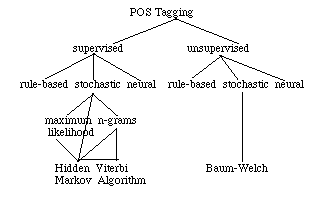
\includegraphics[width=0.7\textwidth]{./images/tagging_overview.png}
  \end{center}
  \caption{Metodi per il PoS-Tagging automatizzato.}
  \label{fig:feedforwardNeuralNetwork}
\end{figure}

\subsection{Supervisionato vs. non supervisionato}
\nocite{BrillMarcus:1993}
\nocite{Brill:1995}
\nocite{Schutze:1993}

Una delle prime distinzioni sugli algoritmi di PoS tagger esistenti pu\`o essere
fatta in base al grado di automazione dei processi di addestramento e classificazione.
I termini comunemente utilizzati per questo tipo di distinzione sono \emph{supervisionato}
e \emph{non supervisionato}.

I classificatori supervisionati sono tipicamente basati su corpus gi\`a taggati.
Questi fungono da base per creare qualsiasi strumento da usare durante tutto il
processo di classificazione. Ad esempio: il dizionario del classificatore, la
frequenza parola/tag, la probabilit\`a di una sequenza di classi e/o l'insieme
di regole per la classificazione.

I modelli non supervisionati, d'altro canto, non hanno bisogno di corpus taggati
bens\`i usano sofisticati algoritmi di computazione per creare gruppi di parole
(in altre parole, classi di parole), per poi utilizzare questi gruppi auto generati
per calcolare le informazioni probabilistiche necessarie ad un classificatore
stocastico oppure per generare le regole di contesto necessarie ad un classificatore
basato su regole.

Il motivo principale per prediligere un metodo completamente automatizzato (e
quindi non supervisionato) al PoS tagging \`e che questo risulta essere estremamente
portabile. \`E risaputo, inoltre, che i classificatori automatici (supervisionati)
tendono a performare meglio se addestrati e testati su una stessa tipologia di
testi di quanto non possano fare i metodi completamente automatizzati.

Sfortunatamente, di corpus gi\`a taggati non ne esistono molti, soprattutto se
si pensa alla moltitudine di lingue che possono richiedere una classificazione
di questo tipo. Anzi, il desiderio di automatizzare questo processo nasce proprio
dalla necessit\`a di classificare con precisione testi che non sono stati classificati,
in virt\`u del fatto che questo processo, se fatto manualmente, comporta un grande
dispendio di tempo e risorse.

Tuttavia, l'approccio completamente automatizzato al PoS tagging porta con se
altri incovenienti. In particolare, i gruppi generati automaticamente da questi
algoritmi, tendono ad essere molto grossolani e spessi si perde quella distinzione
granulare che si trova in quei tag set appositamente studiati per un determinato
linguaggio e utilizzati nei metodi supervisionati.

\subsection{Tagging basato su regole}
\nocite{Brill:1992}
\nocite{Greene:1971}

Di solito, gli approcci basati su regole usano informazioni di contesto per
assegnare una classe a parole sconosciute o ambigue. Queste regole, di solito,
sono conosciute come regole \emph{context frame}.

Ad esempio, una regola di questo tipo pu\`o essere qualcosa del genere: se una
parola $X$ ambigua/sconosciuta \`e preceduta da un \emph{determinante} ed e
seguita da un \emph{nome}, allora $X$ \`e un aggettivo.

In aggiunta a queste informazioni di contesto, molti classificatori utilizzano
informazioni di natura morfologica come aiuti nel processi di disambiguazione.
Una di queste regole potrebbe essere: se la parola ambigua/sconosciuta termina
con il suffisso \emph{-ing} ed \`e preceduta da un verbo, allora etichettala come
verbo (questo ovviamente \`e valido solo per l'inglese)

Alcuni sistemi si spingo anche oltre l'uso di informazioni morfologiche e contestuali,
includendo regole che tengono conto anche della punteggiatura e della capitalizzazione.
Informazioni di questo tipo possono essere di grande o poca utilit\`a, in base
al linguaggio il cui testo dev'essere classificato. Per il tedesco, ad esempio,
le informazioni riguardo la capitalizzazione delle lettere si \`e dimostrata
essere estremamente utile nella classificazione di nomi sconosciuti.

I classificatori basati su regole molto spesso richiedono un addestramento di
tipo supervisionato. Tuttavia, recentemente, \`e aumentato l'interesse nei
confronti dell'induzione automatica di regole.

Un approccio alla induzione automatica di regole consiste nel far classificare,
ad un classificatore, del testo non classificato. Un essere umano, poi, analizza
il risultato della classificazione e corregge ogni parola erroneamente classificata.
Il testo, correttamente classificato, viene poi dato nuovamente in input al
classificatore, che impara le regole di correzione confrontando i due insiemi di
dati.

A volte \`e necessario ripetere questo processo pi\`u volte.

\subsection{Tagging stocastico}

Il termine ``tagger stocastico'' pu\`o essere utilizzato per indicare una grande
variet\`a di approcci al problema del PoS tagging. Infatti, ogni modello che, in
qualche modo, utilizza il concetto di probabilit\`a o frequenza pu\`o essere
etichettato correttamente come stocastico.

Il classificatore stocastico pi\`u semplice, disambigua le parole solamente in
base alla probabilit\`a che una determinata parola occorra con un particolare tag.
Quindi, per una determinata parola, il tag incontrato pi\`u di frequente nel
training set, sar\`a anche quello assegnato a quella parola nel caso in cui la
sua classificazione in un determinato contesto fosse ambigua.

Il problema con questo approccio \`e che, nonostante possa di certo restituire
un tag valido per una data parola, pu\`o anche restituire una sequenza di tag del
tutto non corretta.

Un'alternativa all'approccio basato sulla frequenza delle coppie parola/tag
consiste nel calcolare la probabilit\`a dell'occorrenza di una data sequenza di
tag. Di solito, ci si riferisce a questo approccio con il termine \emph{n-gram},
il nome \`e dovuto al fatto che il tag migliore per una data parola viene
determinato dalla probabilit\`a condizionata che questo occorra dati gli \emph{n}
tag precedenti.

L'algoritmo pi\`u comune per implementare l'approccio n-gram \`e conosciuto come
\emph{Algoritmo Viterbi}. Si tratta di un algoritmo di ricerca che evita
l'espansione polinomiale di una ricerca per ampiezza ``potando'' l'albero di
ricerca ad ogni livello usando le migliori $n$ \emph{Stime di Massima Verosimiglianza}
(dove $n$ rappresenta il numero di possibili tag della parola seguente).

Il livello di complessit\`a successivo che pu\`o essere introdotto in un
classificatore stocastico combina entrambi gli approcci precedenti, usando sia
la probabilit\`a di una sequenza di tag che le misure della frequenza delle parole.
Questo approccio \`e conosciuto come \emph{Hidden Markov Model}.
Ogni stato nascosto di un tag produce una parola nella frase.

Le assunzioni alla base di questo modello sono le seguenti.

\begin{itemize}
  \item Ogni parola non \`e correlata con nessuna delle altre parole della frase
        e i rispettivi tag
  \item La probabilit\`a che una parola sia taggata in un determinato modo dipende
        dagli $n$ tag precedenti.
\end{itemize}

\subsection{Parole sconosciute}

Un problema rimane ancora in sospeso in relazione agli approcci descritti fino
ad ora: come ci si dovrebbe comportare con le parole sconosciute? Alcune delle
regole di un classificatore basato su regole sono in grado di gestire questo
problema, ma cosa accade in un modello stocastico? Come \`e possibile calcolare
la probabilit\`a che una data parola occorra con un dato tag, se quella parola e
sconosciuta al classificatore?

Ci sono diversi possibili soluzioni a questo problema.
Uno consiste nell'usare informazioni di tipo morfologico.
In questo caso il classificatore calcola le probabilit\`a che un determinato
suffisso, appartenente ad una parola sconosciuta, possa presentarsi con un
particolare tag.

Un'altra soluzione consiste nell'assegnare, alla parola sconosciuta, un insieme
di tag predefiniti (di solito si usa Nome, Verbo, Aggettivo e Avverbio), poi si
cerca di disambiguare la parola usando la probabilit\`a che tale classe occorra
dell'n-gram preso in considerazione.

Ancora, un'altra possibilit\`a \`e quella di calcolare la probabilit\`a che ogni
tag del tag set ha di presentarsi alla fine dell'n-gram di riferimento, e di
selezionare la classe con la probabilit\`a pi\`a alta. Tuttavia questa non \`e
la soluzione ottimale, soprattutto quando si utilizza un tag set molto grande.

\subsection{Tokenizzazione}

Il flusso di caratteri di un testo scritto in linguaggio naturale dev'essere
necessariamente diviso in unit\`a di testo distinte e significative (detti token)
prima che un qualsiasi tipo di processamento del linguaggio, che vada oltre il
livello del carattere, possa essere eseguito. Questo processo prende il nome di
\emph{tokenizzazione}

Se un linguaggio \`e perfettamente punteggiato, la tokenizzazione \`e una cosa
semplice da fare: un programma potrebbe estrarre parole e punteggiatura dal testo
semplicemente dividendolo ad ogni spazio bianco e segno ti punteggiatura.

Ma nessun linguaggio reale \`e perfettamente punteggiato, e la situazione \`e
sempre pi\`u complicata di cos\`i. Anche in linguaggi ben (ma non perfettamente)
punteggiato, come l'inglese, ci sono casi in cui la corretta tokenizzazione non
pu\`o essere determinata semplicemente conoscendo la classificazione individuale
di ciascun singolo carattere oltre a casi in cui sono possibili pi\`u tokenizzazioni
per una stessa porzione di testo.

Ad esempio consideriamo la stringa, in inglese, ``\emph{chap.}'' . Questa pu\`o
essere interpretata sia come l'abbreviazione della parola \emph{chapter} che come
la parola \emph{chap} alla fine di una frase. Stessa cosa per la stringa ``\emph{Jan.}'',
pu\`o essere interpretata sia come abbreviazione di \emph{January} che come il
nome proprio \emph{Jan} alla fine di una frase.

Nel primo caso, il punto dev'essere considerato come parte del token mentre nel
secondo caso dovrebbe essere considerato come un token a parte.

Nonostante lo spazio sia un indicatore abbastanza affidabile per individuare i
confini dei token, ci sono parole, in inglese, che sono composte da pi\`u termini
separate da uno spazio (ad esempio \emph{to and for}, \emph{jack rabbit},
\emph{General Motors}, \emph{a priori}).

Tutte queste difficolt\`a incontrate in un linguaggio come l'inglese sono
relativamente limitate e alcune applicazioni di text-processing semplicemente le
ignorano o le affrontano con algoritmi fatti ad hoc.

Ma tutte queste considerazioni sono state fatte su un solo linguaggio, altri
linguaggi presentano problemi simili. L'italiano, ad esempio, usa l'\emph{elisione}
per gli articoli \emph{lo} e \emph{la}, quando questi incontrino una parola
iniziante per vocale. Il tedesco scrive i \emph{nomi composti}, ossia nomi formati
dall'unione di pi\`u parole, senza spazi: \emph{Computerlinguistik} (linguistica
computazionale).

Altri linguaggi offrono sfide ben pi\`u serie. Il cinese, ad esempio, risulta
essere scarsamente punteggiato e la forma pi\`u comune di cinese continentale
non ha spazi bianchi e non \`e segmentato in alcun modo (come il greco che sulla
stele di Rosetta). Inoltre nel cinese la segmentazione \`e ambigua: due caratteri
possono essere trattati come distinti ed avere un significato, oppure come un unico
token ed averne un altro.

\`E evidente come il problema della tokenizzazione sia un problema fortemente
dipendente dal linguaggio e va risolto caso per caso.
